
This chapter answers RQ2 with a controlled experiment over three label sources and a fourth added later (\S{}5.1--\S{}5.6), then follows the source paper's robot-planning chain one link further, asking whether the label source changes the plan an LLM planner produces (\S{}5.7).

\section{The controlled experiment}

RQ2 asks whether the automatic labels are good enough to \textit{train} a relation model as effectively as human labels. The experiment isolates exactly that variable: one lightweight classifier per predicate (a small MLP over pure geometric pair features: relative position, depth difference, box geometry, size-relative gap, mask-contact fractions), trained with \textbf{identical features, architecture, seeds, positive-oversampling and group split}, then evaluated against the \textbf{held-out human gold} (annotator groups 6--8, whose data influenced no threshold, no calibration, and no training). The only difference between the runs is the supervision source. (Training uses a fixed 60-iteration budget for every classifier; some do not fully converge, identically for every source; the comparison is between supervision signals under equal compute, not between tuned models.)

Three sources are compared in the core experiment, because two would leave the obvious objection unanswered; a fourth was added afterwards and is introduced alongside the result it produced (\S{}5.2).

\begin{itemize}
\item \textbf{Human.} The \textasciitilde{}10\% of ordered pairs the annotators chose to label.
\item \textbf{Automatic.} Every pair the tool's rules fire on: dense and
rule-consistent.
\item \textbf{Self-trained (pseudo-labelled).} The rival remedy from the
semi-supervised literature (\S{}2.4), implemented and not argued about. A teacher is trained on the human labels exactly as in the human arm; it then predicts the \textit{unannotated} training pairs, its confident predictions (probability $\geq$ 0.90 either way) become pseudo-labels, and a student is retrained on the union of real and pseudo labels (Lee, 2013). A pair the annotators touched at all counts as labelled, since their silence on its other predicates is informative; a pair they never recorded is the unlabelled pool. This arm answers the question a reader should ask before accepting the project's premise: if the human labels are too sparse, why not simply stretch them?
\end{itemize}

Each source labels the same pairs its own way, and each model inherits its source's character. That contrast is the experiment.

\section{Result}

Averaged over three seeds (42/43/44); each cell shows mean (min--max):

\begin{center}
\small
\begin{longtable}{>{\raggedright\arraybackslash}p{0.135\textwidth}>{\raggedleft\arraybackslash}p{0.140\textwidth}>{\raggedleft\arraybackslash}p{0.140\textwidth}>{\raggedleft\arraybackslash}p{0.140\textwidth}>{\raggedleft\arraybackslash}p{0.140\textwidth}>{\raggedleft\arraybackslash}p{0.135\textwidth}}
\caption{Downstream recall against held-out human gold for the three label sources.}\\
\hline
predicate & human-trained & self-trained & vision-language & auto-trained & gold (held-out) \\
\hline
\endfirsthead
\hline
predicate & human-trained & self-trained & vision-language & auto-trained & gold (held-out) \\
\hline
\endhead
on & 0.84 (0.83--0.86) & 0.90 (0.89--0.92) & 0.76 (0.68--0.89) & 0.88 (0.87--0.89) & 348 \\
under & 0.44 (0.36--0.53) & 0.59 (0.59--0.60) & 0.84 (0.71--0.91) & 0.85 (0.85--0.85) & 192 \\
to the left of & 0.22 (0.18--0.29) & 0.31 (0.27--0.34) & 0.42 (0.41--0.43) & 0.95 (0.95--0.95) & 446 \\
to the right of & 0.25 (0.22--0.31) & 0.38 (0.37--0.39) & 0.35 (0.30--0.44) & 0.99 (0.99--0.99) & 550 \\
in front of & 0.09 (0.08--0.10) & 0.12 (0.12--0.13) & 0.08 (0.07--0.09) & 0.19 (0.19--0.19) & 609 \\
behind & 0.15 (0.12--0.17) & 0.22 (0.17--0.28) & 0.21 (0.21--0.23) & 0.37 (0.37--0.37) & 580 \\
near & 0.08 (0.00--0.19) & 0.03 (0.00--0.06) & 0.00 (0.00--0.00) & 1.00 (1.00--1.00) & 93 \\
\textbf{mean} & \textbf{0.30} & \textbf{0.36} & \textbf{0.38} & \textbf{0.75} &  \\
\hline
\end{longtable}
\end{center}

A fourth arm answers what \S{}4.13 raises but cannot settle: if a vision-language model is not a good enough \textit{annotator}, is it a good enough \textit{teacher}? The same model labelled all 600 training images, used exactly as the other three sources are. Every arm trains on precisely the pairs that arm covers, so none is advantaged by seeing more of the split, and the human, self-trained and automatic figures are unchanged from the three-arm experiment to the last decimal, which is the check that this is an addition, not a different experiment. The answer is a qualified yes: at 0.38 the vision-language labels teach better than the sparse human labels they would replace and about as well as the standard remedy for scarce labels, while remaining half as useful as computed geometry.

Figure~\ref{fig:rq2-with-vlm} draws the four arms per predicate. Training on the automatic labels multiplies downstream mean recall by \textasciitilde{}2.5 against the human annotators' own held-out labels: 0.75 vs 0.30. Self-training lands between the two but far closer to the floor: it improves the human baseline on six of seven predicates and lifts the mean to 0.36, which closes \textbf{15\% of the distance} between the human and automatic arms. Stretching the existing labels helps; it does not substitute for labelling every pair consistently.
\begin{figure}[!htbp]
\centering
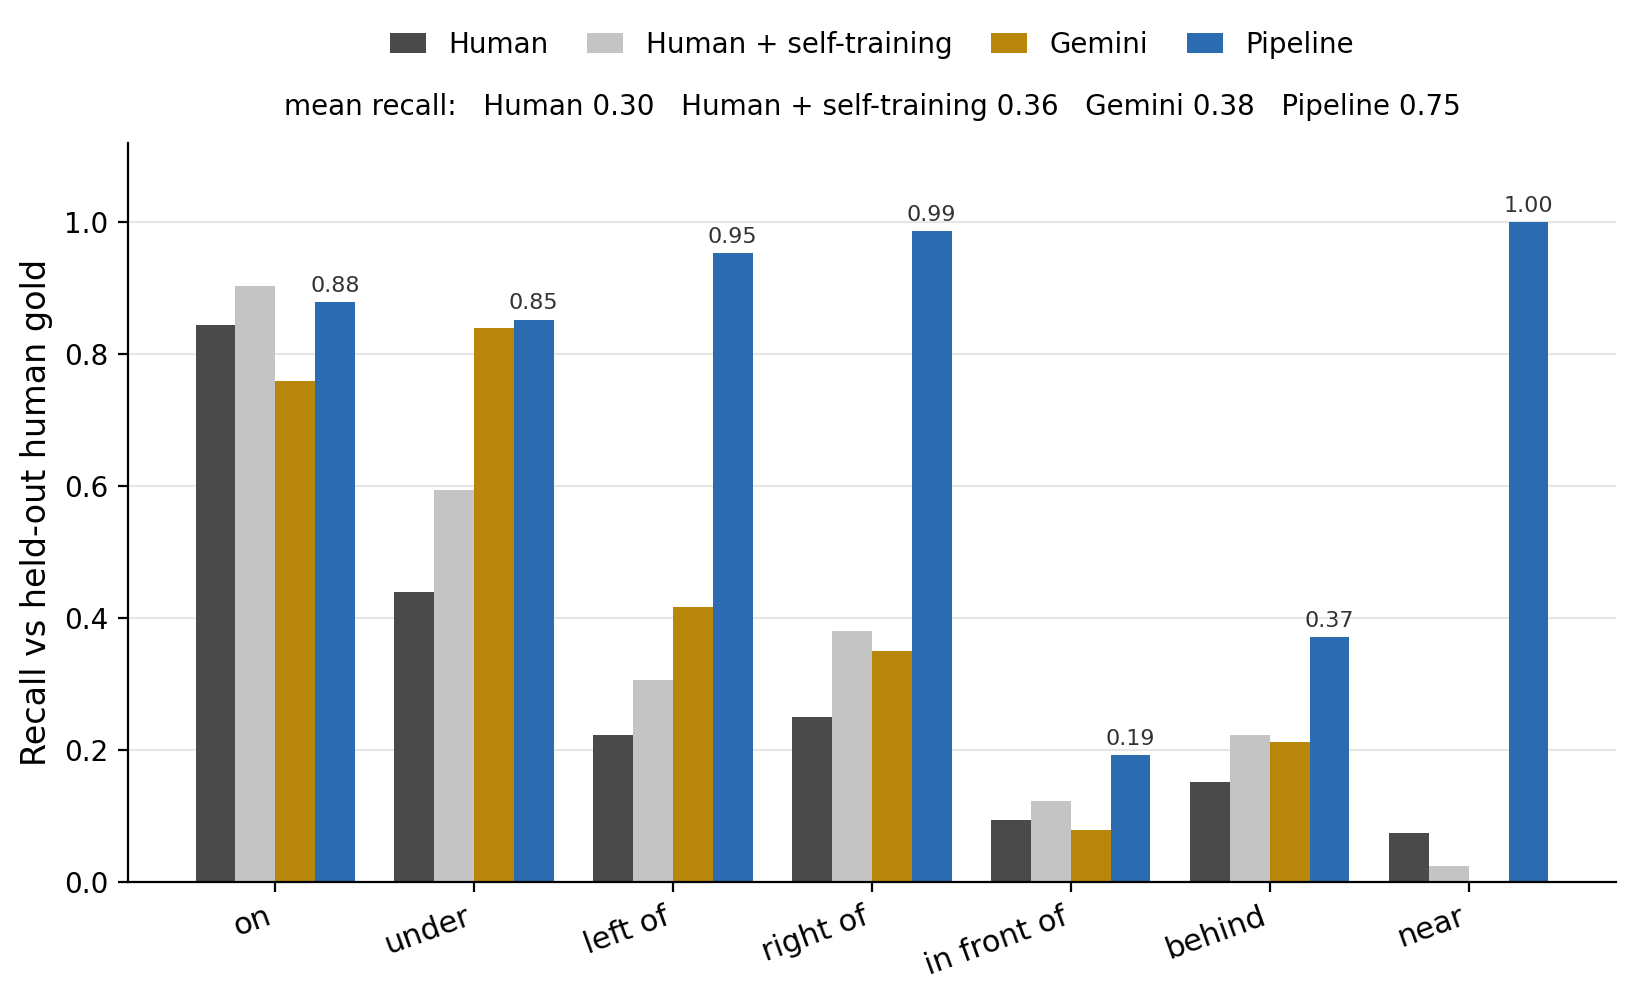
\includegraphics[width=0.80\textwidth]{figures/rq2-with-vlm.png}
\caption{Downstream recall against held-out human gold by label source. Every arm trains on the same pairs, so the label source is the only variable. Self-training improves on the human labels everywhere except \texttt{near}, where it falls below them.}
\label{fig:rq2-with-vlm}
\end{figure}


The seed spreads carry a second result. The auto-trained model's recall varies by at most 0.02 across seeds on every predicate, while the human-trained model's varies by up to 0.19 (\texttt{near} spans 0.00--0.19) and the self-trained model inherits that instability (\texttt{behind} spans 0.17--0.28). Sparse supervision is not just weaker, it is \textit{unstable}, its outcome hostage to sampling noise, and self-training passes the instability on to its student.

\subsection{The same experiment on four other indicators}

A recall-only table invites one obvious objection: the automatic arm labels twenty times more densely, so of course it recovers more. The objection is answered by measurement, and the answer is not the flattering one. \textbf{On every indicator except recall the automatic arm comes last}: macro precision 0.136 against the human arm's 0.252, F1 0.194 against 0.267, average precision 0.164 against 0.230, and micro F1, which weights predicates by how often the annotators used them, harshest of all at 0.066 against 0.262. Taken at face value the table says the automatic labels are the worst supervision of the four.

They are not, and one number shows why. Average precision is threshold-free, so no arm improves it by committing to more pairs, and the automatic arm still scores **0.040 on *to the left of***, the predicate on which \S{}4.4 audited fifteen of its fifteen extra predictions and found every one correct. An arm cannot be both wrong and right about laterality. What the column measures is agreement with which pairs an annotator chose to write down, so this is the artefact of \S{}4.3 reappearing one level down the chain, and it charges the denser arm for the coverage that makes it useful. The columns cannot be argued away in the automatic arm's favour either, since \S{}4.4 audited the \textit{rule layer's} extra predictions and not the classifier's. Appendix F.5 gives the full table and both readings.

What the four indicators establish is narrower than the recall column suggests and firmer than the precision column implies: judged on the labels' ability to teach a model to recover relations humans recorded, the automatic arm dominates; judged on its ability to imitate which relations humans chose to record, it does not, and no metric computed against this gold can separate the two.


\section{Why self-training does not rescue the human labels}

The pseudo-label arm's own bookkeeping explains its ceiling precisely. Of the 60,762 training pairs, the annotators recorded just \textbf{6,026}. Filling in the rest, the teacher adds roughly \textbf{54,000 confident negative} pseudo-labels per predicate against only \textbf{36 to 67 confident positives}: a ratio of about 1,000 to 1. The teacher, trained on annotation in which most pairs carry no label, has learned above all that pairs usually have no relation, and self-training feeds that conviction back to the student as though it were evidence. What propagates is not the annotators' knowledge but their silence.

This is the failure mode \S{}2.4 predicted from the literature, now measured. Pseudo-labelling is well behaved when the labelled seed is a representative sample of the unlabelled pool. Here it is neither representative nor complete: the annotators labelled the pairs they found salient, so absence of a label conflates "no relation holds" with "nobody looked". A student trained on the union cannot distinguish the two, and inherits a systematic bias towards silence.

The \texttt{near} row makes the point sharply. Human-trained recall is already at near-collapse, 0.08, and self-training pushes it \textit{down} to 0.03: only three of nine annotator groups used the label, so the teacher's notion of "near" is both weak and idiosyncratic, and its confident pseudo-labels bury what little positive signal existed. Where the seed is defective, self-training does not merely fail to help, it amplifies the defect. The comparison is therefore not "programmatic labels beat doing nothing" but "programmatic labels beat the standard remedy, under identical conditions, closing more than six times as much of the available gap". Active learning is not tested because it fails for a simpler reason (\S{}2.4): it still buys human labels, so it lowers the bottleneck's cost without removing it.

\section{Why the automatic labels win, and two consistency checks}

The mechanism is the one measured throughout. A classifier trained on labels that are sparse (\textasciitilde{}10\% of pairs) and inconsistent (\S{}4.5, \S{}4.7) learns above all to be silent, and its recall collapses exactly where labelling was thinnest (\texttt{near} 0.08, lateral 0.22--0.25); trained on dense rule-consistent labels the same model learns the geometry (near 1.00, lateral 0.95--0.99, support 0.85--0.88). That is \S{}2.3's weak-supervision prediction confirmed under controlled conditions. Two checks argue the result is real, not an artefact: the auto-trained model's profile almost exactly reproduces the rule layer's own held-out performance (mean 0.75 against the rules' 0.74; front/behind 0.19/0.37 against the rules' 0.20/0.37), so the classifier \textit{distilled the annotator}, which is what "the labels are learnable" means; and all three arms face identical features, the same oversampling cap and the same held-out gold, including the convention-inverted annotators, which penalises every arm's front/behind equally.


\section{Boundaries of the claim}

The evaluation gold is itself sparse human annotation, so recall is primary, mirroring RQ1, and \S{}5.2.1 shows why none of the other columns reads as an error rate here. The human-trained model's weakness is partly a property of \textit{any} sparse supervision at this scale, and more human labels would improve it, but producing them is the bottleneck this project removes and the self-trained arm shows the shortfall cannot be computed away instead. The front/behind rows are depressed for every arm by the held-out groups' inverted convention (Chapter 4), so the penalty is shared.

One structural caveat needs stating plainly. The classifier's features are geometric and the automatic labels come from rules over closely related geometry, so the auto-trained arm is partly re-learning its own generator. Read alone, this chapter shows the automatic labels are \textit{learnable} and the human labels are not, and not that they win under any featurisation. Three things keep it meaningful: every arm gets identical features; being learnable is itself the property RQ2 asks about, since a downstream consumer must extract a consistent signal; and Chapter 6 removes the circularity by repeating the comparison in a full scene-graph model with visual features.

\section{From labels to robots: where this sits in the source paper's chain}

The source paper's end goal is explicit: spatial understanding exists so that robots can plan. Their motivating example shows an LLM planner failing to remove a cube before grasping the book beneath it until SGG-derived relations are supplied, after which it "generates executable, spatially-aware plans." The paper's own evaluation of that chain stops at SGG quality: six models benchmarked on the human labels, topping out at mR@100 = 0.49 (VCTree), with every model saturating by epoch 2--6 and \texttt{near} stuck at 0.22--0.25 (\S{}2.2).

Each symptom has a cause this dissertation measured and a remedy it built. Saturation within six epochs is what training on the 8,926 sparse triplets of \S{}4.2 looks like, and the automatic labels give 20$\times$ the supervision on the same images. The universal \texttt{near} failure is what an undefined, three-annotator label looks like, and the fitted-threshold labels are perfectly learnable (this chapter's proxy reaches 1.00). The depth predicates were being taught two opposite conventions; the automatic labels apply one. Three predictions follow, registered here before the direct test that judges them in Chapter 6: later saturation, a higher plateau, and the recovery of \texttt{near}.

\section{The planner experiment: does the label source change what a robot would do?}

Section 5.6 ends with the source paper's motivating example, in which an LLM planner fails to remove a cube before grasping the book beneath it until spatial relations are supplied. The paper asserts it on one scene. It can be run as an experiment, and this section runs it.

\textbf{Design.} Twenty-five held-out scenes were selected in which a target object has a second object resting on it, so any safe plan must move the occluder first. Each scene is put to an LLM planner three times, in prompts differing only in what they state: \textbf{A} lists the objects and nothing else, \textbf{B} adds the human-annotated relationships, \textbf{C} adds the automatically computed ones. One filter runs over both relation conditions first, so no relation is offered to one planner that would have been withheld from the other; density is deliberately not equalised, since matching a sparser source would mean throwing away true relations. A plan is safe if it moves the occluder before the step that grasps the target, judged by published rules and not by reading (\texttt{eval/score\_\allowbreak{}planner.py}), so scoring is blind by construction and a reader who disputes a verdict can inspect the rule. Appendix E.5 gives the filter, the prompt construction, the scene-level forensics and a scoring defect that hand-reading caught. The experiment was run twice, on \texttt{gemini-flash-latest} and on the reasoning model \texttt{gemini-3.1-pro-preview}, and two further conditions were added on the larger planner only: \textbf{D} replaces the tool's relations with the vision-language model's from \S{}4.13, and \textbf{E} supplies the union of C and D.

\begin{center}
\small
\begin{longtable}{>{\raggedright\arraybackslash}p{0.125\textwidth}>{\raggedright\arraybackslash}p{0.372\textwidth}>{\raggedright\arraybackslash}p{0.202\textwidth}>{\raggedleft\arraybackslash}p{0.185\textwidth}}
\caption{Planner experiment: whether the plan clears the occluding object before grasping the target, over 25 held-out scenes under each label source.}\\
\hline
Condition & Prompt states & Safe plans (flash) & Safe plans (pro) \\
\hline
\endfirsthead
\hline
Condition & Prompt states & Safe plans (flash) & Safe plans (pro) \\
\hline
\endhead
A & objects only & 0 / 25 & 0 / 25 \\
B & human relationships & 25 / 25 & 25 / 25 \\
C & automatic relationships & 19 / 25 & 19 / 25 \\
D & vision-language relationships & not run & 20 / 25 \\
E & automatic and vision-language combined & not run & \textbf{25 / 25} \\
\hline
\end{longtable}
\end{center}

Figure~\ref{fig:planner-sources} shows the five conditions side by side. The two planners agree exactly, and not merely in the totals: the six scenes C fails on are scenes 1, 4, 16, 19, 24 and 25 under \textit{both} models. A finding that survives replacing the reasoning engine, down to which scenes fail, is a property of the information in the prompt, not of the model consuming it, which is the claim the experiment exists to make. It also disposes of the objection to condition A's zero, that a more capable planner would infer support from the object list: it does not, in twenty-five scenes out of twenty-five, twice. The failure without relations is more specific than inattention, since in seven of the A plans the planner \textit{names} the occluder but only as something to steer around, treating something resting on the target as a neighbour to avoid, not a load to remove.
\begin{figure}[!htbp]
\centering
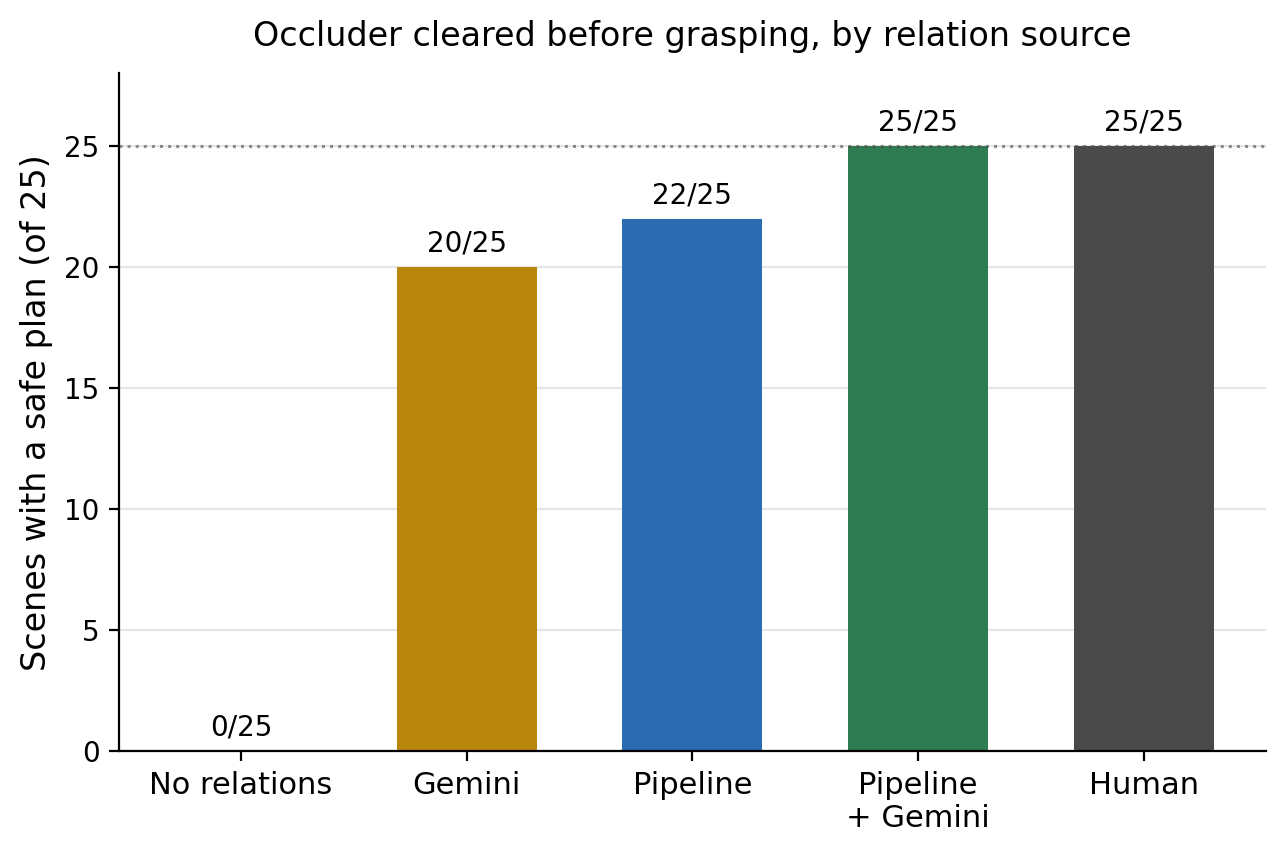
\includegraphics[width=0.80\textwidth]{figures/planner-sources.png}
\caption{Scenes with a safe grasp plan, by the relation source given to the planner. Neither automatic source matches human annotation alone, and under the shipped support threshold the vision-language source is marginally ahead of the geometric one; their union matches it, because their failures are disjoint.}
\label{fig:planner-sources}
\end{figure}


\textbf{The two automatic sources fail on different scenes, and the union closes the gap.} Condition D scores 20 of 25 against the tool's 19, so under the shipped rule the vision-language source is marginally the stronger of the two alone. What matters is the structure underneath: C fails on scenes 1, 4, 16, 19, 24 and 25, D on 3, 5, 6, 13 and 14, and \textbf{the two sets do not intersect}. Every failure in both arms is a support relation the source did not supply, never a plan that reasoned badly from what it was given, so a union supplying more support relations repairs exactly those cases and cannot break the ones already working. It does: condition E clears the occluder in all 25 scenes, drawing level with the human labels, and gains six scenes over condition C while losing none. This is the only measurement here on which automatic labels \textit{match} human annotation on a robot-relevant task instead of approaching it, with no human in the labelling loop.

All six C failures have the same cause, and it is not a planning failure: the automatic relation list did not contain the support relation. The occluder was described accurately in every way except the one the task depended on, and in zero cases was the support relation present and ignored. The converse is nearly but not quite true: seven scenes lack the relation and six fail, scene 7 being recovered from the surrounding description alone. Six misses in twenty-five scenes is 24\%, against the measured support recall of 0.81/0.75 in \S{}4.2 and the refit that traded recall for precision in \S{}4.14, so the planner result is the fidelity result showing up one level higher in the chain --- and it moves when that fidelity does.

\textbf{Twenty-five scenes is small, and the pairing is what makes it enough.} Every condition is put to the same scenes, so the evidence sits in the scenes where two conditions disagree, and an exact McNemar test over those (\texttt{eval/planner\_\allowbreak{}paired\_\allowbreak{}tests.py}) says which comparisons this sample can settle. It settles the ones the argument rests on. Supplying relations at all separates from supplying none, 25 discordant scenes for the human labels and 19 for the tool's, all in one direction, p < 10\textasciicircum{}-5. The union's gain over the tool alone is 6 scenes to 0, p = 0.031, as is the human arm's lead over the tool alone, the comparison that runs against this project.

The same test names what 25 scenes cannot settle. The tool against the vision-language source is 6 discordant scenes to 5, p = 1.00, so the two-scene margin means nothing and this section declines to read it; the union's edge over that source alone, 5 to 0, reaches only p = 0.063. The paired tests are also sharp exactly where the absolute rates are not: C's own rate is 19 of 25 with a 95\% interval of [0.55, 0.91]. This experiment measures \textit{which source is better on these scenes} far more precisely than how often any of them would succeed in general, and that generalisation is weak because of what the scenes are, not how many.

\textbf{What this does not show.} The scenes were selected to contain an occluder, so the result speaks to that situation and not to task planning at large. The vision-language model's assertions were never audited as the tool's were (\S{}4.4), so the union's gain is measured on the planning task alone. The comparison is between label sources and not planners: condition B is handed the exact fact the task tests. And no robot moved, so this measures plans, not executions, and closes the gap between labels and robot behaviour by one link rather than entirely.

\textbf{The threshold refit of \S{}4.14 cost condition C three scenes, and E none.} An earlier version of this experiment ran on the labels \texttt{on\_\allowbreak{}contact\_\allowbreak{}min} 0.60 produced and recorded C at 22 of 25. The shipped rule is 0.85, which emits support more sparingly: across the same 25 scenes the support relation the task depends on is now present in 18, not 22, absent in scenes 1, 4, 7, 16, 19, 24 and 25 where before it was absent in 4, 16 and 24 alone. Re-run on the shipped labels, \textbf{C scores 19 of 25 on both planners} and E still scores 25 of 25, with 6 scenes gained over C and none lost.

That the two planners again agree exactly, and at a different value from before, is the same evidence the earlier agreement gave: what the prompt contains decides the outcome, and which engine consumes it does not. C recovers one scene more than the count of available support relations would predict, so absence of the relation is nearly but not quite sufficient for failure; \texttt{grasps\_\allowbreak{}target} and \texttt{no\_\allowbreak{}invented} remain 1.00 throughout, so no plan failed for any other reason.

\textbf{The complementarity result strengthens under the stricter rule.} The seven scenes the tool now misses and the five the vision-language model misses are still \textbf{disjoint}, so their union supplies a support relation for all 25. Tightening the geometric source widened its own gap by three scenes and left the union closing every one of them, which is a harder test of the same claim than the original passed.

One further limitation is structural and worth stating plainly, because it bounds what the result can mean. \textbf{The scoring rule cannot see a false positive.} It asks whether the plan moves the occluder before grasping the target, so a support relation the tool asserts wrongly costs an unnecessary step, not a failed plan. Section 4.14 measures those at 0.40 precision, and this experiment is insensitive to them by construction: it tests whether the labels carry \textit{enough}, not whether they carry \textit{too much}. A task penalising wasted motion, or one where moving the wrong object is unsafe, not merely inefficient, would rank these label sources differently, and nothing here predicts how.

What it settles is the question \S{}5.6 could only frame. The tool's relations alone carry 76\% of the decision-relevant content human labels carry on this task, against 0\% for no labels at all, and combined with the vision-language model's they carry all of it. The residual gap in the single-source arm is not a property of computed labels in general but of one predicate whose recall is measured, whose precision was refitted, and whose failure modes are diagnosed in \S{}4.9 and \S{}4.14 --- which is why tightening that predicate moved this number and moved nothing else in the chapter.


\section{Answer to RQ2}

Yes, with more than was asked. At this dataset's scale of human annotation the automatic labels are not merely "good enough" but \textbf{substantially better training material than the human labels themselves}, because density and consistency dominate raw human authority when supervision is sparse. The self-trained arm rules out the cheap alternative: the standard semi-supervised remedy recovers only 15\% of the gap, because it propagates the annotators' silence, not their knowledge. That is the dissertation's core claim, that removing the bottleneck can \textit{grow} dataset utility instead of approximating it, demonstrated on the dataset's own held-out annotators and against the obvious rival.